\documentclass{tran-l}

\usepackage{enumerate}
\usepackage{amsfonts}
\usepackage{cancel}
\usepackage{amssymb}
\usepackage{amsthm}
\usepackage[all]{xy}
\usepackage{hyperref}
\usepackage{todonotes}

\usepackage{multicol}
\usepackage{pifont}
\newcommand{\cmark}{\ding{51}}
\newcommand{\xmark}{\ding{55}}
\newcommand{\hmark}{\ding{119}}

\newtheorem{theorem}{Theorem}[section]
\newtheorem{lemma}[theorem]{Lemma}

\theoremstyle{cor}
\newtheorem{cor}[theorem]{Corollary}

\theoremstyle{definition}
\newtheorem{definition}[theorem]{Definition}
\newtheorem{example}[theorem]{Example}
\newtheorem{xca}[theorem]{Exercise}

\theoremstyle{remark}
\newtheorem{remark}[theorem]{Remark}

\theoremstyle{conjecture}
\newtheorem{conjecture}[theorem]{Conjecture}


\newcommand{\p}{\mathfrak{p}}
\newcommand{\supp}{\text{supp}}
\newcommand{\onto}{\twoheadrightarrow}



\numberwithin{equation}{section}

\DeclareMathOperator{\Hom}{\text{Hom}}
\DeclareMathOperator{\rad}{\text{rad}}
\DeclareMathOperator{\characteristic}{\text{char}}
\DeclareMathOperator{\grade}{\text{grade}}
\DeclareMathOperator{\lcm}{\text{lcm}}
\DeclareMathOperator{\rank}{\text{rank}}
\DeclareMathOperator{\eltht}{\text{height}}
\DeclareMathOperator{\littlerank}{\text{little rank}}
\DeclareMathOperator{\Ext}{\text{Ext}}

\begin{document}

\title{Uniformly Most Powerful Tests for \\ Ad Hoc Transactions in Monero}



\author{B G Goodell}
\address{Cypherstack}
\curraddr{}
\email{brandon@cypherstack.com}
\thanks{}

\author{Rigo Salazar}
\address{Cypherstack}
\curraddr{}
\email{rigo@cypherstack.com}
\thanks{}

\author{Freeman Slaughter}
\address{Cypherstack}
\curraddr{Department of Mathematical and Statistical Sciences, Clemson University}
\email{freeman@cypherstack.com}
\thanks{}

\date{}

\dedicatory{}

\begin{abstract}
We introduce a general, low-cost, low-power statistical test for transactions in transaction protocols with small anonymity set authentication (TPSASAs), such as Monero.
The test classifies transactions as \textit{ad hoc} (spontaneously constructed to spend a deterministically selected key) or \textit{self-churned} (constructed from a probability distribution very close to that of the default wallet software, and with the same sender and receiver).
The test is a uniformly most powerful (UMP) likelihood ratio tests (LRT) from the Neyman-Pearson Lemma, and makes no assumptions about user behavior.
We extend these tests to expoit prior information about user behavior.
We discuss test parameterization, as well as how anonymity set cardinality and user behavior impact test performance.
We also describe a maximum-likelihood de-anonymization attack on Monero based on our test.
\end{abstract}

\maketitle

\section{Introduction}

Output-based transaction protocols (TPs) verifiably authenticate transactions with digital signatures (\cite{nakamoto2008bitcoin}, \cite{buterin2013ethereum}).
With digital signatures, public keys are directly linkable with corresponding signatures, so it is simple to directly trace the chain of custody of funds.
On the other hand, some TPs instead introduce \textit{spender ambiguity} by authenticating transactions with anonymity sets of public keys, e.g.\ via ring signatures as in the original CryptoNote protocol (\cite{van2013cryptonote}) or zero-knowledge proofs (\cite{hopwood2016zcash}, \cite{eagen2022zero}).
Tracing the chain of custody of funds through anonymity sets with cardinality $n$ requires computing correct paths through a directed acyclic graph where each node has $n$ children, which is thought to be more difficult as $n$ increases (and $n=1$ is the non-ambiguous case).

Unfortunately, when these anonymity sets are small, transactions leak information about user behavior, e.g.\ via so-called EAE attacks (\cite{breaking_monero_poisoned_outputs}, \cite{ali2024scaling}), allowing attackers to gain advantage at tracing funds.
\textit{Self-churn}, a folklore mitigation to these leaks, is the practice of punctuating real transactions with sequences of simulated transactions where the sender and receiver are the same (\cite{meiklejohn2013fistful}, \cite{chator2023practice}, \cite{ranshous2017exchange}, \cite{yang2019behavioral}, \cite{Pernice2021Cryptocurrencies}).
We call these intermediate simulated transactions \textit{churn transactions}.
On the other hand, real transactions are typically made \textit{ad hoc} by spending one or more deterministically selected outputs.

The distributions of \textit{ad hoc} transactions and churn transactions are different enough to build statistical tests exploiting the gap.
We introduce a general statistical test which classifies transactions in TPs with small anonymity set authentication (TPSASAs, e.g.\ as in Monero via ring signatures) as \textit{ad hoc} or churned.
We call this the \textit{basic test} for \textit{ad hoc} transactions.
The basic test is a uniformly most powerful (UMP) likelihood ratio test (LRT), due to the Neyman-Pearson lemma \cite{neyman1933ix}.
Assuming a prior distribution describing user behavior and/or more sophisticated default wallet software, similar approaches yield \textit{extended tests} for \textit{ad hoc} transactions.
The existence of these tests represent a tremendous security threat for users of TPSASAs, even when these tests have low power.

Our basic test is low cost and has variable, but generally low, power, and is related to previous attacks.
Our extended tests are similarly low cost but can attain greater power by violating uniformity of the basic test.
Test parameterization is generally very expensive, must be re-computed in the event of a blockchain re-organization, and must be re-computed regularly as the blockchain grows.
Prototype python code for parameterizing our tests by estimating critical values of harmonic means of sets of random variables sampled from mixed distributions is available at this paper's repository on GitHub at \url{https://www.github.com/cypherstack/churn}.

Test power responds strongly to variations in the statistical distance between user-selected distributions and default wallet distributions, explaining practical security improvements since \cite{moser2017empirical}, \cite{miller2017empirical}.
Test power responds weakly to variations in anonymity set size, so increasing anonymity set sizes is not an effective mitigation.
Our tests have no practical utility in protocols with very large anonymity sets (e.g.\ ZK-SNARKs in \cite{hopwood2016zcash} or full-chain membership proofs in in \cite{eagen2022zero}).
Our tests have no practical utility when user behavior is very well-described by the default wallet distribution, whether due to low prevalence of \textit{ad hoc} transactions or similarity between user behavior and the default wallet distributions.
Unfortunately, if user behavior is very different from the default wallet distribution, prevalence of \textit{ad hoc} transactions must be low before the basic test loses its practical utility.

\subsection{Organization}

This paper is organized as follows. In Section \ref{sec:preliminaries}, we set out preliminary notation and background. In Section \ref{sec:basic_test}, we derive our basic test and describe its extensions. In Section \ref{sec:basic_parameterization}, we discuss the parameterization of our basic test. In Section \ref{sec:test_attack}, we discuss tracing attacks against TPSASAs using our tests. In Section \ref{sec:discussion}, we discuss our results. In Section \ref{sec:conclusion_and_future}, we draw some conclusions and make notes on directions for future work.


\section*{Changes}



This paper is part of an open, iterative research process and will be regularly updated, with each revision accompanied by a detailed changelog.
Future versions will include expanded analyses, new findings, numerical parameterization, additional experimental results, refinements to our formal models and their practical applications, corrections, and more.
We use version control via GitHub at \url{https://www.github.com/cypherstack/churn}.
The following describes changes made to this document since 21 October 2024.
\begin{itemize}
\item 21 October 2024. Initial draft.
% \item \today. Some future changes.
\end{itemize}

\section{Preliminaries and Notation}\label{sec:preliminaries}

We use $\approx$ informally as ``approximately equal,'' not to indicate statistically negligible differences.

Let $\epsilon > 0$.
Let $n, m, d \in \mathbb{N}$.
For any subset $T \subseteq S$, define the set complement $\overline{T} = \left\{s \in S \mid s \notin T\right\}$ as usual.
Let $I$ be the boolean indicator function, such that $I(P) = 1$ when proposition $P$ is true and $I(P) = 0$ otherwise.
For some real numbers $x_1, \ldots, x_n$, denote the tuple $\underline{x} = (x_1, \ldots, x_n)$ and, for any function $f$ with domain $\text{dom}(f) \subseteq \mathbb{R}^n$, denote $f(\underline{x}) = (f(x_1), \ldots, f(x_n))$.
Define the harmonic mean $H(\underline{x}) = n \left(\sum_{i=1}^{n} x_i^{-1} \right)^{-1}$ and the log harmonic mean $h(\underline{x}) = \ln(H(\underline{x}))$.


A probability mass function (PMF) on a finite set $S$ is a function $f: S \to [0,1]$ such that $\sum_{s \in S} f(s) = 1$.
We say a random variable $X$ has PMF $f$ if $\mathbb{P}[X=s] = f(s)$.
Note that, generally, if $f$ is a PMF on $S$, the function we denoted $f(\underline{s}) = (f(s_1), \ldots, f(s_n))$ is not a PMF.


We follow usual likelihood principles (\cite{casella2024statistical}) as follows.
For a parameter space $\Theta$, subset $\Theta_0 \subseteq \Theta$, an element $\theta \in \Theta$, and a random variable $X$ which takes on values in some set $\mathcal{X}$, and let $R \subseteq \mathcal{X}$ be a region. Then $R$ corresponds to the rejection region of an inferential statistical test for a hypothesis that $\theta \in \Theta_0$.

A type I error occurs when $\theta \in \Theta_0$ yet $x \in R$.
The probability of a type I error is the \textit{size} $\alpha = \mathbb{P}_{\theta}[x \in R \mid X = x, \theta \in \Theta_0]$.
The complement of the size $1-\alpha$ is the \textit{specificity} of the test.
An upper bound on the size $\alpha$ a \textit{level} of the test.

A type II error occurs when $\theta \notin \Theta_0$ and $x \notin R$.
The probability of a type II error is the \textit{miss rate} $\beta = \mathbb{P}_{\theta}[x \notin R \mid X = x, \theta \notin \Theta_0]$.
The complement of the miss rate $1-\beta$ is the \textit{power} or \textit{sensitivity} of the test.




\begin{lemma}[Neyman-Pearson]
Let $A \subseteq \Theta$ be a negligible set, $\theta_0, \theta_1 \in \Theta$ such that $\theta_0 \neq \theta_1$, $\alpha \in (0, 1)$, and $k \in (0, \infty)$.
For an unknown $\theta \in \Theta$, let $\mathcal{H}_0$ be the hypothesis that $\theta = \theta_0$, and let $\mathcal{H}_1$ be the hypothesis that $\theta = \theta_1$.
If $R$ is the rejection region for $\mathcal{H}_0$ corresponding to this test such that
\begin{itemize}
\item $x \in R \setminus A$ implies $\mathbb{P}[X=x \mid \theta = \theta_0] < k\mathbb{P}[X=x \mid \theta = \theta_1]$, and
\item $x \in \overline{R} \setminus A$ implies $\mathbb{P}[X=x \mid \theta = \theta_0] > k\mathbb{P}[X=x \mid \theta = \theta_1]$,
\end{itemize}
then the test has size $\alpha$, is UMP in the set of level $\alpha$ tests, every UMP test in the set of level $\alpha$ tests also satisfies these conditions with the same $k$ (but possibly different sets $A$), and every UMP test in the set of level $\alpha$ tests agrees with the others except possibly on their corresponding negligible sets $A$.
\end{lemma}


We say that the test is \textit{parameterized} by $k$.
Given a distribution for a random variable $X$ with parameter space $\Theta$, we define the usual \textit{likelihood function} as \[\mathcal{L}(\theta^\prime \mid x) = \mathbb{P}\left[X=x \mid \theta = \theta^\prime\right]\]
and, given subset $\Theta_0 \subseteq \Theta$, we  define the \textit{likelihood ratio} as follows. \[\Lambda(x) = \frac{\sup_{\theta^\prime \in \Theta_0} \mathcal{L}(\theta^\prime \mid x)}{\sup_{\theta^\prime \in \Theta} \mathcal{L}(\theta^\prime \mid x)}\]
The likelihood ratio is a metric for the likelihood that $\mathcal{H}_0$ is true. Thus, rejection region $R$ in the Neyman-Pearson lemma satisfies the following.
\begin{itemize}
\item Small likelihood is necessary to reject $\mathcal{H}_0$: $x \in R \setminus A$ implies $\Lambda(x) < k$.
\item Large likelihood is necessary to accept $\mathcal{H}_0$: $x \in \overline{R} \setminus A$ implies $\Lambda(x) > k$.
\end{itemize}


Let $\mathcal{Y}$ be a finite set of public keys for a TPSASA (the entire key space).
Let $y^* \in \mathcal{Y}$ be an unknown, fixed element.
In the sequel, let $f$ be a PMF on $\mathcal{Y}$ from default wallet software, which is used to sample anonymity set members.

We assume that the wallet distribution $f$ is not dependent upon $y^*$.
This assumption is not valid, in general, but in practice, $f$ is usually only dependent upon the time at which the transaction was constructed, which we can approximate by proxy with the time the transaction appeared.
Moreover, our approach below can be immediately modified so that $f$ depends on $y^*$; we describe these modifications as we go.
This, also, is not a valid assumption, in general, as users may sign a transaction offline and wait a period of time before relaying it on the network.
However, this is a rather unusual occurrence given the typical use-case of permissionless e-cash, which we describe below.

\section{Basic Test for Churn}\label{sec:basic_test}



\subsection{Ad Hoc Anonymity Sets}\label{sec:basic_test_ad_hoc_transactions}

The usual use-case for permissionless e-cash is an \textit{ad hoc} transaction.
The user owns some fixed, unknown $y^* \in \mathcal{Y}$ and decides that $y^*$ must be spent, so they do the following.
\begin{enumerate}
\item Sample a distinguished index $1 \leq i^* \leq d$ with the default wallet software.
\item Set $y_{i^*} = y^*$.
\item For each $1 \leq i \leq n$ such that $i \neq i^*$, independently sample $y_i \in \mathcal{Y}$ with PMF $f$ employed by the default wallet software, re-sampling in the case of collisions. Then the tuple $\underline{y} = (y_1, \ldots, y_n)$ can be interpreted as an $n$-set.
\item Use $\underline{y}$ as the anonymity set to authorize the transaction.
\end{enumerate}

Consider observing $\underline{y}$ conditioned upon the event that this anonymity set comes from an \textit{ad hoc} transaction spending $y^*=y_{i^*}$ for an unknown index $i^*$.
The probability of this occurrence can be computed with the law of total probability and modeling the index $i^*$ corresponding to $y^*$ with a uniform random variable $J$ on $\left\{1, \ldots, n\right\}$.
\begin{align}
\mathbb{P}[\underline{y}] =& \sum_{j=1}^{n} \mathbb{P}[\underline{y} \mid J = j] \mathbb{P}[J= j] \\
=& n^{-1} \sum_{j=1}^{n} \mathbb{P}[\underline{y} \mid J = j]  \\
=& n^{-1} \sum_{j=1}^{n} \mathbb{P}[\underline{y} \mid y_j = y^*] \\
=& n^{-1} \sum_{j=1}^{n} \prod_{\substack{i = 1 \\ i \neq j}}^n f(y_i) \label{eqn:pmf_ad_hoc}
\end{align}

If the distribution $f$ depends on $y^*$, there exists some family of PMFs $f_{y}$ on $\mathcal{Y}$ and parameterized by $y \in \mathcal{Y}$ such that $\mathbb{P}[\underline{y} \mid y_j = y^*] = \prod_{i=1, i \neq j}^n f_{y_j}(y_i)$. The same approach works without the assumption that $f$ does not depend on $y^*$ (but our resulting basic test no longer is a UMP).
In this case, we just obtain the following.
\begin{align}\mathbb{P}[\underline{y}] = n^{-1} \sum_{j=1}^{n} \prod_{\substack{i=1 \\ i \neq j}}^n f_{y_j}(y_i)\end{align}
We only use Equation \ref{eqn:pmf_ad_hoc} in the sequel for simplicity of our analysis.

\subsection{Churn Anonymity Sets}\label{sec:basic_test_churn_transactions}

Churn transactions, on the other hand, are not just \textit{ad hoc} transactions with the same sender and receiver, since $y^*$ may be unlikely to appear in a random transaction.
Indeed, churn transactions have anonymity sets $\underline{y}$ distributed like a sample of $n$ elements without replacement from the default wallet PMF $f$.
In particular, we must have $\mathbb{P}\left[\left\{y_1, \ldots, y_n\right\}\right] = f(y_1)f(y_2) \ldots f(y_n)$.
However, $f(y^*)$ is not entirely within the user control.
In practice, $f$ and $\mathcal{Y}$ evolve over time, and anonymity sets in transactions are typically sampled only a (relatively) brief time before the transaction is broadcast. Thus the equality may be relaxed slightly to approximate equality.
\begin{align}
\mathbb{P}\left[\underline{y}\right] \approx f(y_1)f(y_2) \ldots f(y_n) \label{eqn:pmf_churn}
\end{align}

Default wallet distributions $f$ are not unimodal in practice, because they are locally sensitive to blockchain density. However, $f$ does tend to be approximately unimodal with respect to the age of elements of $\mathcal{Y}$.
So, if $y^*$ is sufficiently young, then the user can wait a random period of time such that the observed $f(y^*)$ is not unusual-looking before constructing an otherwise \textit{ad hoc} transaction.
In this case, the transaction does not appear to have a real signer, and therefore the simulation cannot reveal anything about the true signer $i^*$.

To approximate a churn transaction, beginning at a secret time $t$ and ending at time $t^\prime$, users may employ the following approach.
\begin{enumerate}
\item Independently sample some $\tilde{y}$ with PMF $f$ and compute secret $u = f(\tilde{y})$.
\item Discard $\tilde{y}$ safely and keep $u$ secret.
\item Wait until a future time such that $f(y^*) \approx u$, then immediately construct the transaction with the \textit{ad-hoc} approach from the previous section.
\item Discard $u$ safely.
\end{enumerate}
The resulting sample $\underline{y}$ appears to be sampled from the wallet PMF.
If an observer learns of $u$ and/or the starting time $t$, they gain an advantage in distinguishing that the transaction is a churn transaction.
If $f$ is unimodal with respect to the age of elements of $\mathcal{Y}$ and $y^*$ is not sufficiently young for this churn procedure to work, the user cannot spend $y^*$ in a churn as described.
Unfortunately, this forces the user to spend $y^*$ as an \textit{ad hoc} transaction.
However, if this \textit{ad hoc} transaction is to oneself, the user receives a new $y^\prime$ which is sufficiently young to be subsequently spent in a churn transaction.

Just as before, we can consider the case that $f$ depends on $y^*$.
We again use the law of total probability, an independent uniform random variable $J$ on $\left\{1, 2, \ldots, n\right\}$.
\begin{align}
\mathbb{P}[\underline{y}] =& \sum_{j=1}^{n} \mathbb{P}[\underline{y} \mid y_j = j^*] \mathbb{P}[J=j^*] \\
=& n^{-1}\sum_{j=1}^n \prod_{i=1}^n f_{y_j}(y_i)
\end{align}

However, in the sequel, we use Equation \ref{eqn:pmf_churn} for simplicity of our analysis.


\subsection{Distribution of Anonymity Sets}\label{sec:basic_test_distribution}

We model the distribution of anonymity sets with the following PMF $g$ with parameter space $\Theta = \left\{0,1\right\}$ with parameter $\theta \in \Theta$.
\begin{align}
\label{eqn:main} g_\theta(\underline{y}) = \mathbb{P}_\theta[\underline{y}] =& (1-\theta)\prod_{i =1}^n f(y_i) + \frac{\theta}{n} \sum_{j=1}^{n} \prod_{i \neq j} f(y_i)\\
g_0(\underline{y}) = \mathbb{P}_{\theta=0}[\underline{y}]  =&  \prod_{i =1}^n f(y_i) \\
g_1(\underline{y}) = \mathbb{P}_{\theta=1}[\underline{y}] =& \frac{1}{n} \sum_{j=1}^{n} \prod_{i \neq j} f(y_i)
\end{align} where $\theta = 0$ corresponds to a churn transaction and $\theta = 1$ corresponds to an \textit{ad hoc} transaction.



\subsection{Test Statistic for Basic Test}\label{sec:basic_test_test_statistic}


Now to test the null hypothesis $\mathcal{H}_0$ that $\theta = 0$ against the alternative hypothesis $\mathcal{H}_1$ that $\theta = 1$ with the Neyman-Pearson Lemma, we have the following likelihood function and likelihood ratio.
\begin{align}
\label{eqn:likelihood} \mathcal{L}(\theta \mid \underline{y}) =& g_\theta(\underline{y}) = \mathbb{P}_\theta[\underline{y}] \\
=& (1-\theta)\prod_{i =1}^n f(y_i) + \frac{\theta}{n} \sum_{j=1}^{n} \prod_{i \neq j} f(y_i) \\
\label{eqn:likelihood_ratio} \Lambda =&
\frac{\mathcal{L}(0 \mid \underline{y})}{\max\left\{\mathcal{L}(0 \mid \underline{y}), \mathcal{L}(1 \mid \underline{y})\right\}}
= \frac{g_0(\underline{y})}{\max\left\{g_0(\underline{y}), g_1(\underline{y})\right\}} \\
=& \begin{cases} 1; & g_0(\underline{y}) > g_1(\underline{y}) \\ \frac{\prod_i f(y_i)}{n^{-1} \sum_j \prod_{i \neq j} f(y_i)}; & g_0(\underline{y}) \leq g_1(\underline{y})
\end{cases}\\
=& \begin{cases} 1; & g_0(\underline{y}) > g_1(\underline{y}) \\ H(f(\underline{y})); & g_0(\underline{y}) \leq g_1(\underline{y})
\end{cases}
\end{align}
Thus, our test statistic is just the harmonic mean of probabilities of the sample under $f$, $H(f(\underline{y}))$.

That the harmonic mean appears here may be surprising.
The harmonic mean is biased towards the smallest element of a sample.
If a sample of probabilities has a small harmonic mean, the sample must therefore have at least one small probability.
In this way, the Neyman-Pearson lemma just formalizes the notion that the test statistic is small when at least one element of the sample $\underline{y}$ does not appear to have been sampled independently from $f$, i.e.\ $\mathcal{H}_0$ appears to be unlikely.


\subsection{Computing PMF}

To compute our test statistic requires computing $f(y)$ for various values of $y \in \mathcal{Y}$, where $f$ is the PMF implied by the default wallet decoy selection algorithm.
The function $f$ is generally not easy to derive in a closed-form solution, even with access to default wallet source code.
However, we can follow a few general rules to obtain a model for $f(y)$ which is sufficient for practical testing.

Recall $\mathcal{Y}$ is a description of the keys available for use as anonymity set members on the blockchain, $\mathcal{Y}$ has a structure imposed by the blockchain.
In particular, there is a partition of $\mathcal{Y}$, one part for each block.
The parts of this partition are linearly orderable by block height, and these different blocks have different cardinalities.
The linear order can be interpreted as a clock, and for a given block $B_i$, we refer to the average number of keys per block in blocks close in time to $B_i$ as the \textit{blockchain density} at height $i$.
Generally, for any $y \in B_i$, $f(y)$ is inversely proportional to blockchain density at height $i$.

Also, $f(y)$ is also dependent on the age of $y$, in terms of block height when $y$ was mined.
Since \cite{moser2017empirical}, it has been popular to empirically estimate the distributions of ground-truth spend-times, modeling these as Gamma-distributed random variables (which can be thought of as sums of exponentially-distributed random variables).
Spend-time is a continuous random variable, whereas a sampled block on the blockchain is a discrete random variable, however, and the discrete analogue of the exponential random variable is the geometric random variable.
Since a sum of geometric random variables is a negative binomial random variable, we can model $f(y)$ as proportional to a negative binomial PMF, $\mathbb{P}[k] = \binom{k+r-1}{k}(1-p)^kp^r$, for some parameters $r > 0$ and $p \in (0,1)$. If these parameters are not specified directly in the default wallet software, they can be estimated using standard statistical inference techniques and samples from the default wallet software.

Hence, if we denote the local blockchain density near $y$ with $\texttt{density}(y)$, the age of $y$ in $\mathcal{Y}$ in terms of block height with $\texttt{age}(y)$, we have $f(y) \approx \frac{\binom{\texttt{age}(y)+r-1}{\texttt{age}(y)}(1-p)^\texttt{age}(y) p^r}{\texttt{density}(y)}$.


\subsection{The Basic Test}\label{sec:basic_test_corollary}


The Neyman-Pearson Lemma intuitively rejects the hypothesis that the data was generated with parameter $\theta = 0$ if the likelihood that $\theta = 0$ is much smaller than the likelihood that $\theta = 1$.
Note that the only negligible subset of $\left\{0,1\right\}$ is the empty set.


\begin{cor}
Let $\alpha \in (0, 1)$, $c \in (0, \infty)$, $\underline{y} \in \mathcal{Y}^n$. For an unknown $\theta \in \left\{0,1\right\}$, let $\mathcal{H}_0$ be the hypothesis that $\theta = 0$ and let $\mathcal{H}_1$ be the hypothesis that $\theta = 1$. If $R$ is the rejection region for $\mathcal{H}_0$ corresponding to this test such that
\begin{itemize}
\item $\underline{y} \in R$ implies $\mathbb{P}[\underline{y} \mid \theta = 0] < k\mathbb{P}[\underline{y} \mid \theta = 1]$, and
\item $\underline{y} \notin R$ implies $\mathbb{P}[\underline{y} \mid \theta = 0] > k\mathbb{P}[\underline{y} \mid \theta = 1]$,
\end{itemize} then the test has size $\alpha$, is UMP in the set of level $\alpha$ tests, every UMP test in the set of level $\alpha$ tests also satisfies these conditions with the same $k$, and every UMP test in the set of level $\alpha$ tests  agrees with the others.
\end{cor}

A rejection region which satisfies these conditions is $R = \left\{\underline{y} \mid kg_1(\underline{y}) > g_0(\underline{y})\right\}$.
This region has a corresponding significance $\alpha = \mathbb{P}\left[\underline{y} \in R \mid \theta = 0\right] = \sum_{\underline{y} \in R} g_0(\underline{y})$, the resulting test has size $\alpha$ and is UMP in the set of tests with level $\alpha$.
Rewriting $kg_1(\underline{y}) > g_0(\underline{y})$ as $\Lambda = \frac{g_0(\underline{y})}{g_1(\underline{y})} < k$, we have the following rejection region
\[R = \left\{\underline{y} \mid H(f(\underline{y})) < k\right\} = \left\{\underline{y} \mid h(f(\underline{y})) < h_\alpha\right\}\]
where $h_\alpha = \ln(k)$ parameterizes the test at size $\alpha$.
This provides a one-sided test which rejects $\mathcal{H}_0$ whenever the (log) harmonic mean of the probabilities of occurrence is sufficiently small.

To run the basic test, the following is sufficient.
\begin{itemize}
\item Evaluate $f$ $n$ times.
\item Compute $n$ inversions of floating point numbers.
\item Compute a mean of these $n$ floating point numbers.
\item Invert a floating point number.
\item Comparing two floating point numbers.
\end{itemize}

If evaluating $f$ takes time at most $t_f$, inverting a floating point number takes time at most $t_{\text{inv}}$, computing a mean of $n$ floating point numbers takes time at most $t_{n,\text{mean}}$, and comparing two floating point numbers takes time $t_{\text{comp}}$, then the test takes time $O(n \cdot t_f + (n+1)t_{\text{inv}} + t_{n, \text{mean}} + t_{\text{comp}})$.


As we shall see, evaluating the wallet distribution $f$ is, itself, a nontrivial challenge; see Section \ref{sec:wallet_distro} for a discussion.

\subsection{Extensions}\label{sec:basic_test_extended}


Attackers may utilize additional knowledge about user behavior to develop non-uniform tests with better performance than our basic UMP LRTs.
Indeed, exchanges and large economic actors with detailed ground-truth knowledge of user identities and locations can leverage these data.
Such an actor could use the distribution $g_1$ from our basic test as a Bayesian prior, and uses their ground-truth knowledge to compute an update to develop a new prior $\hat{g}_{1}$, one for each user.
Of course, for every user, most of $\hat{g}_1$ is fixed by the default wallet distribution, and we have
$\hat{g}_{1}(\underline{y}) = \sum_{j=1}^{n} \hat{f}(y_j) \prod_{i \neq j} f(y_i)$ for some $\hat{f}$ associated with the user. Thus we obtain the distribution
\begin{align}
\hat{g}_\theta(\underline{y}) =& (1-\theta) \prod_i f(y_i) + \frac{\theta}{n}\sum_j \hat{f}(y_j) \prod_{i \neq j} f(y_i) \\
=& \hat{\mathcal{L}}(\theta \mid \underline{y})\\
\hat{\Lambda} =& \frac{\hat{\mathcal{L}}(0 \mid \underline{y})}{\max\left\{\hat{\mathcal{L}}(0 \mid \underline{y}), \hat{\mathcal{L}}(1 \mid \underline{y})\right\}} = \frac{\hat{g}_0(\underline{y})}{\max\left\{\hat{g}_0(\underline{y}), \hat{g}_1(\underline{y})\right\}} \\
=& \frac{\prod_i f(y_i)}{n^{-1} \sum_j \hat{f}(y_j) \prod_{i \neq j} f(y_i)}\\
=& H\left(\frac{f(y_1)}{\hat{f}(y_1)}, \frac{f(y_2)}{\hat{f}(y_2)}, \ldots, \frac{f(y_n)}{\hat{f}(y_n)}\right)
\end{align}
Following the same reasoning as for the basic test, we reject the null hypothesis $\mathcal{H}_0$ that $\theta=0$ whenever $\hat{\Lambda}$ is sufficiently small.
We have the following rejection region \[R = \left\{\underline{y} \mid H\left(\frac{f(y_1)}{\hat{f}(y_1)}, \ldots, \frac{f(y_n)}{\hat{f}(y_n)}\right) < k \right\} = \left\{\underline{y} \mid h\left(\frac{f(y_1)}{\hat{f}(y_1)}, \cdots, \frac{f(y_1)}{\hat{f}(y_n)}\right) < h_{\alpha}\right\}\] where $h_{\alpha} = \ln(k)$ parameterizes the test for size $\alpha$, providing a similar one-sided test to the basic test.


To run the extended test, the following is sufficient.
\begin{itemize}
\item Evaluate $f$ and $\hat{f}$ $n$ times each.
\item Compute $n$ inversions of floating point numbers.
\item Compute $n$ products of floating point number pairs.
\item Compute a mean of these $n$ products.
\item Invert a floating point number.
\item Comparing two floating point numbers.
\end{itemize}

If evaluating $\hat{f}$ takes time $t_{\hat{f}}$, computing a product of two floating point numbers takes time $t_{\text{mul}}$, then the extended test takes time $O(n \cdot (t_f + t_{\hat{f}} + t_{\text{mul}}) + (n+1)t_{\text{inv}} + t_{n, \text{mean}} + t_{\text{comp}})$.


\section{Basic Test Parameterization and Power}\label{sec:basic_parameterization}




To apply this test with a given $\alpha$, we require a value $h_{\alpha}$ such that $\alpha = \mathbb{P}_{\theta=0}\left[\underline{y} \in R\right] = \mathbb{P}_{\theta=0}\left[h(f(\underline{y})) < h_\alpha\right]$.
An estimate of $h_{\alpha}$is possible without any additional assumptions or ground-truth data.
We explain the general approach in this section.

See Figure \ref{fig:rejection_region} for a diagram showing the idea for an arbitrary unimodal distribution on $h \in \mathbb{R}_{< 0}$.
The shaded region is the rejection region for the size $\alpha$ UMP LRT basic test for churn, where the dashed line is the critical value $h=h_\alpha$. The harmonic mean of elements from $(0,1)$ is an element from $(0,1)$, so $h < 0$, explaining the domain of Figure \ref{fig:rejection_region}.
Since anonymity set members are sampled from a finite set, our test statistic is a discrete random variable, but the general picture also applies for densities.


In the case of densities, the critical value $h_{\alpha}$ is the exact value such that $\alpha = \mathbb{P}_{\theta=0}\left[h(f(\underline{y})) < h_\alpha \mid \mathcal{H}_0\right]$; equivalently, the area of the shaded region is exactly $\alpha$.
In the case of mass functions, $h_{\alpha} = \sup\left\{\ln(k) \mid \mathbb{P}_{\theta=0}\left[h(f(\underline{y})) < \ln(k) \mid \mathcal{H}_0\right] \leq \alpha \right\}$; equivalently, the area of the shaded region is as close to $\alpha$ as the distribution allows without exceeding $\alpha$.
\begin{figure}[h]\label{fig:rejection_region}
\centering
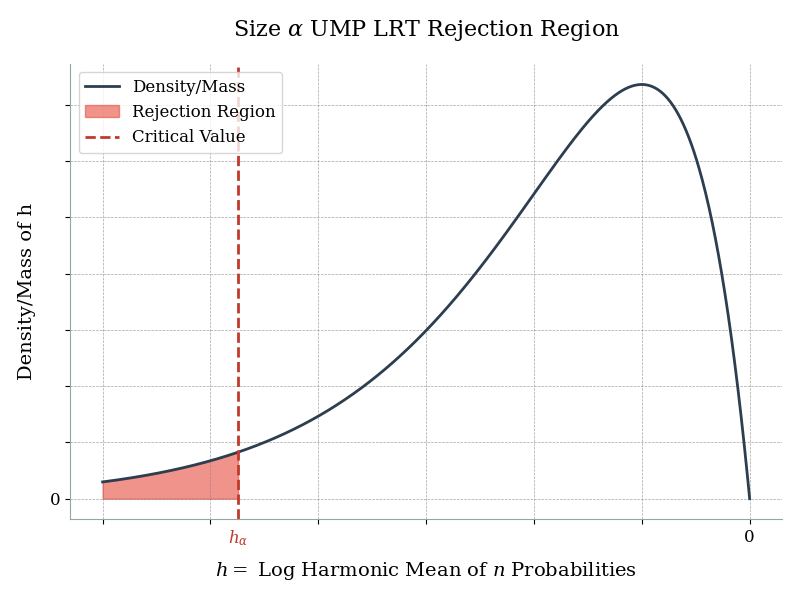
\includegraphics[width=\textwidth]{rejection_region}\caption{Illustrative sketch of a possible PMF (or PDF) for the log harmonic mean of $n$-tuples of probabilities under the null hypothesis $\mathcal{H}_0$; this is only a sketch, and should not be expected to resemble the ground-truth.
}
\end{figure}


\subsection{Suggested Empirical Approach}

The distribution of $h(f(\underline{y}))$, conditioned upon $\underline{y}$ being sampled from $f$, is sensitive to the distribution of $f(\underline{y})$ under this same condition.
No model of the distribution of the values $f(y)$ conditioned upon $y$ being sampled from $f$ is immediately obvious.
An empirical distribution of $f(y)$ from Monte Carlo approaches is easily obtainable, though, from which we can estimate the $100\alpha$-th percentile critical value $h_\alpha$ as follows.

We use the fact that the $\ell^{th}$ order statistic in a sample of $m$ observations is an unbiased estimate of the $100 \cdot\frac{\ell}{m+1}$-th percentile critical value, and compute the estimate for $\alpha = \frac{\ell}{m+1}$.
For example, for $\alpha = 0.05$, the classic critical value used in mathematical statistics, set $\ell=1$ and $m=19$.

However, a point estimate for $h_\alpha$ alone does not provide a good description of the precision to which we can represent $h_\alpha$.
To rectify this, we use interval estimation, taking large enough sample sizes to guarantee a decimal representations with some $\kappa \in \mathbb{N}$ digits of precision in using scientific notation.

A popular option for interval estimation is the $100(1-\alpha^*)\%$ confidence interval.
\begin{align}
\left(\overline{h} - t_{\frac{\alpha^*}{2},L-1} \frac{S}{\sqrt{L}}, \overline{h} + t_{\frac{\alpha^*}{2},L-1} \frac{S}{\sqrt{L}}\right)\label{eqn:confidence_interval}
\end{align} where $\overline{h}$ is the sample mean, $L$ is the sample size, $t_{\frac{\alpha^*}{2}, L-1}$ is the $\frac{\alpha^*}{2}$-th critical value for Student's t-distribution with $L-1$ degrees of freedom, and $S$ is the sample standard deviation. This interval contains an independently sampled $\overline{h}$ with probability around $1-\alpha^*$.
However, our task is to find $h_\alpha$ such that, for an independently sampled $\underline{y}$, $\alpha = \mathbb{P}\left[h(f(\underline{y})) < h_\alpha \mid \mathcal{H}_0\right]$. Thus, the $100(1-\alpha^*)\%$ prediction interval in Equation \ref{eqn:prediction_interval} is more appropriate
\begin{align}\left(\overline{h} - t_{\frac{\alpha^*}{2},L-1} S \sqrt{1 + \frac{1}{L}}, \overline{h} + t_{\frac{\alpha^*}{2},L-1} \sqrt{1 + \frac{1}{L}}\right)\label{eqn:prediction_interval}
\end{align} where $\overline{h}$, $L$, $t_{\frac{\alpha^*}{2},L-1}$, and $S$ are all as in Equation \ref{eqn:confidence_interval}.
We suggest the following procedure with multilevel sampling.
\begin{enumerate}
\item Input digits of precision $\kappa \in \mathbb{N}$, tuple length $n \in \mathbb{N}$, desired sizes $\alpha, \alpha^* \in (0,1)$, inner sample size $m \in \mathbb{N}$ such that $\alpha = \frac{\ell}{m+1}$ for some integer $1 \leq \ell \leq m$, and outer sample size $L \in \mathbb{N}$, and the $\frac{\alpha^*}{2}$-th critical value for the $t$ distribution with $L-1$ degrees of freedom, $t_{\frac{\alpha^*}{2}, L - 1}$ .
\item For each $1 \leq i \leq L$, do the following.
\begin{enumerate}
\item For each $1 \leq j \leq m$, sample anonymity set $\underline{y}_{i, j} = \left\{y_{i, j, 1}, \ldots, y_{i, j, n}\right\}$ and compute $h_{i, j} = h(f(\underline{y}_{i, j})$.
\item Compute $h_{i, (\ell)}$, the $\ell^{th}$ order statistic of $\left\{h_{i, 1}, \ldots, h_{i, m}\right\}$, and set $h_i = h_{i, (\ell)}$.
\end{enumerate}
\item Now we have a sample $h_{1}, h_{2}, \ldots, h_{L}$ of $\ell^{th}$ order statistics; we use the fact that the $\ell^{th}$ order statistic is an unbiased estimate of the $100\frac{\ell}{m+1}$-th critical value. Compute the following:
\begin{align}
\overline{h} =& L^{-1} \sum_i h_i \\
S =& \sqrt{\frac{\sum_i (h_i - \overline{h})^2}{L-1}} \\
h_{\texttt{low}} =& \overline{h} - t_{\alpha^\prime/2, L-1} S \sqrt{1 + \frac{1}{L}} \\
h_{\texttt{high}} =& \overline{h} + t_{\alpha^\prime/2, L-1} S \sqrt{1 + \frac{1}{L}}
\end{align}
\item If rounding the significands of the scientific notation representations of $\overline{h}$, $h_{\texttt{low}}$, and $h_{\texttt{high}}$ to $\kappa$ digits does not yield the same result, increase $L$ (say, by doubling the sample size) and repeate the process again.
\item Otherwise, set $h_{\alpha}$ to be this rounded value and terminate.
\end{enumerate}

We make no assumptions about user behavior, using only honestly sampled anonymity sets.
Unfortunately, $f$ evolves as the blockchain evolves, so the critical values $h_{\alpha}$ are sensitive to the state of $\mathcal{Y}$ at the time the transaction appeared.
Thus, the same empirical sampling procedure needs to be repeated at different block heights.
Possibly, this may be optimized by binning blocks into epochs without sacrificing much performance.

This process is guaranteed to terminate, thanks to the law of large numbers and the central limit theorem.
However, by doubling sample sizes repetitively, we risk wastefully oversampling, and by performing test statistic computations which are not rolling computations in between each doubling, we introduce a lot of unnecessary overhead.

While a small optimization to this basic algorithm is to compute $\overline{h}$ in a rolling fashion, we cannot do this with $S$.
Another small optimization is to avoid wastefully oversampling and wasting time on intermediate computations which are not relevant to the final output.
Do this with a small initial sample $L^\prime$ to get initial observations $\overline{h}^\prime$, $S^\prime$, $h_{\texttt{low}}^\prime$, and $h_{\texttt{high}}^\prime$, then estimating an improved sample size $L$ such that a follow-up sample of $L$ elements is very likely to satisfy $\kappa$ digits of precision.


Running this parameterization procedure only needs to be done once for each confirmed block height, and executed again in the case of a block reorganization.
However, the procedure requires taking $L\cdot m \cdot n$ samples of from the wallet distribution $f$, evaluating $f$ on each observation from this sample, computing the corresponding log harmonic means of the $n$-tuples from these samples, and finding the $\ell$-th order statistics from the $m$-tuples of these log harmonic means. Lastly, we compute the mean and sample standard deviation, but this is done once and is very fast compared to all the previous.


Thus, if it takes time $t_{\text{sample}}$ to sample an churned anonymity set with cardinality $n$ from $f$, time $t_f$ to evaluate $f$, time $t_{h}$ to compute the log harmonic mean of an $n$-tuple, and time $t_{\text{ord},k,m}$ to compute the $k$-th order statistic from a sample of $m$ log harmonic means, then it takes about time $O(Lmt_{\text{sample}} + Lmnt_f + Lmt_h + Lt_{\text{ord},k,m})$ to parameterize the scheme.
Thus, once the test is parameterized, the test is very low-cost to execute, and the test only needs to be parameterized once.
However, test parameterization takes $O(Lmn)$ time,
and $L$ generally grows quadratically with required precision.
This, coupled with the fact that test parameterization must be occasionally done as the blockchain grows, test parameterization as described here is much more expensive than running the test itself.

\subsection{Model Selection}


In addition to empirically estimating $h_\alpha$, we can perform goodness-of-fit tests on the empirical distribution of the values $v = f(y)$ to determine useful families models and infer parameters.
Beta-distributed random variables, in particular, are capable of modeling many unimodal distributions on $(0,1)$, and are a good candidate.
Then, numerical integration or Monte Carlo techniques from the model can be used to determine $h_{\alpha}$ similarly as in the previous section, but from the inferred model instead of the empirically observed data.
Indeed, in the previous section, we essentially used Monte Carlo sampling of anonymity sets from $f$ to estimate $h_\alpha$ directly, whereas this approach first determines a model for $v = f(y)$ and uses numerical integration or Monte Carlo techniques from the model instead.
As model selection improves, we expect these two approaches to produce similar results, providing a useful ``reality check.''

Prototype python code for estimating critical values of harmonic means of sets of random variables sampled from mixed distributions is available at this paper's repository on GitHub at \url{https://www.github.com/cypherstack/churn}.
This code focuses on moding these $v$ with beta distributions.




\subsection{Relating Parameterization to Power}\label{sec:basic_parameterization_and_power}


In this section, we relate $\beta$ of our basic test with rejection region $R$ to the test specificity $1-\alpha^\prime$ of a \textit{related} test with a similar rejection region $R^\prime$.

Recall the following.
A type I error occurs when a churned transaction is classified as \textit{ad hoc}; this occurs with probability $\alpha$ and is called a \textit{false positive}.
Test specificity is the true negative rate, which is $1-\alpha$.
These probabilities are selected during parameterization.
A type II error, on the other hand, occurs when an \textit{ad hoc} transaction is classified as churned; this occurs with probability $\beta$, and is called a \textit{false negative}.
Test sensitivity is the true positive rate, also known as test power, which is $1-\beta$.
These probabilities are difficult to estimate without access to ground truth data, generally, but we have the following.

In the case that $\theta = 1$, every $y_i$ for $i \neq i^*$ is sampled via $f$, and the final $y_{i^*} = y^*$ is fixed and unknown. For this fixed unknown $y_{i^*}$, we have a fixed and unknown $v = f(y_{i^*})$. Then, given that $\theta=1$, $H(f(\underline{y})) > k$ if and only if \[\frac{n}{v^{-1} + \sum_{i \neq i^*} f(y_i)^{-1}} > k.\]
Equivalently, $n > \frac{k}{v} + k \sum_{i \neq i^*} f(y_i)^{-1}$.
Since $H(f((y_i)_{i \neq i^*})) = \frac{n-1}{\sum_{i \neq i^*} f(y_i)^{-1}}$, we have that $\sum_{i \neq i^*} f(y_i)^{-1} = \frac{n-1}{H(f((y_i)_{i \neq i^*}))}$, so $H(f(\underline{y})) > k$ if and only if $n > \frac{k}{v} + \frac{k(n-1)}{H(f((y_i)_{i \neq i^*}))}$.
Thus, $n - \frac{k}{v} > \frac{k(n-1)}{H(f((y_i)_{i \neq i^*}))}$, or $H(f((y_i)_{i \neq i^*})) > k\frac{n-1}{n - \frac{k}{v}}$.
For convenience, set $k^\prime = k\frac{n-1}{n - \frac{k}{v}}$ and $\underline{y}^\prime = (y_i)_{i \neq i^*}$.
Note that, where $\underline{y}$ is an \textit{ad hoc} transaction and is therefore sampled with $g_{\theta=1}$, $\underline{y}^\prime$ is, on the other hand, sampled entirely with $f$.

Thus, we have the following key observation: $k^\prime$ parameterizes a rejection region $R^\prime$ for a test which is similar to our basic test, but for anonymity sets with cardinality $n-1$ instead of $n$.
The corresponding test has rejection region \[R^\prime = \left\{\underline{y}^\prime \mid H(f(\underline{y}^\prime)) < k^\prime\right\} = \left\{\underline{y}^\prime \mid H(f(\underline{y}^\prime)) < k\frac{n-1}{n - \frac{k}{v}}\right\}\] and some corresponding probability of a type I error $\alpha^\prime$ determined by the critical test statistic value $k^\prime = k\frac{n-1}{n - k/v}$.
Thus, the probability of a type II error for our basic test is
\begin{align}
\beta =& \mathbb{P}\left[H(f(\underline{y})) > k \mid \theta = 1\right] \\
=& \mathbb{P}\left[H(f(\underline{y}^\prime)) > k^\prime \mid \theta = 0\right]\\
=& \mathbb{P}\left[\underline{y}^\prime \notin R^\prime \mid \theta = 0\right]\\
=& 1 - \alpha^\prime
\end{align}
The size of the related test $\alpha^\prime = \mathbb{P}\left[H(f(\underline{y}^\prime)) > k^\prime \mid \theta = 0\right]$ coincides with the power of our basic test $1-\beta$.



Note $0 < \frac{k}{v}$ always, but $\frac{k}{v} < 1$ or not.
So, we have two cases.
In the first case, $\frac{k}{v} < 1$, so $n - 1 < n - \frac{k}{v} < n$, so $\frac{1}{n} < \frac{1}{n - \frac{k}{v}} < \frac{1}{n-1}$, and $\frac{n-1}{n} < \frac{n-1}{n - \frac{k}{v}} < 1$.
Of course, if $n$ is sufficiently large, $\frac{n-1}{n} \approx 1$, so we must have $\frac{n-1}{n - \frac{k}{v}} \approx 1$.
In particular, when $\frac{k}{v} < 1$ and $n$ is sufficiently large, $k^\prime \approx k$ so $R^\prime \approx \left\{\underline{y}^\prime \mid H(f(\underline{y}^\prime)) < k\right\}$.
Also, the harmonic mean is weighted towards the smallest elements, so when $k < v$ and $n$ is sufficiently large, $H(f(\underline{y}^\prime)) \approx H(f(\underline{y}))$ with high probability.
Thus, in the first case, if our basic test has significance $\alpha$, then our related test will have significance approximately $\alpha$, indicating that our basic test also has power $\alpha$.

In the other case, $1 < \frac{k}{v}$. As $\frac{k}{v}$ gets larger, $\frac{n-1}{n - \frac{k}{v}}$ gets larger, leading to larger rejection regions $R^\prime$ associated with these related tests.
Larger rejection regions $R^\prime = \left\{\underline{y}^\prime \mid H(f(\underline{y}^\prime)) < k^\prime\right\}$ are associated with related tests which more aggressively reject the null hypothesis.
These related tests have increased sizes $\alpha$, and therefore the associated basic tests should have increased power.

Thus, we ought to expect test power to roughly begin at our significance $\alpha$ when $v = f(y^*)$ is large and to increase as $v = f(y^*)$ decreases.
In particular, we ought to expect that test power is greatest against the least-likely $y^* \in \mathcal{Y}$ to be sampled under the default wallet distribution $f$.

\subsection{Parameterization of Extensions}

The extended test uses the test statistic $H\left(\frac{f(y_1)}{\hat{f}(y_1)}, \ldots, \frac{f(y_n)}{\hat{f}(y_n)}\right)$. Finding $h_\alpha$, then, requires some knowledge of $\hat{f}$, the distribution selected by the user.
Given this additional information, parameterization can proceed nearly identically as in the previous sections.

Unfortunately, while $v=f(y)$ may be well-described by Beta distributed random variables, the corresponding value from the extended test $r=\frac{f(y)}{\hat{f}(y)}$ generally cannot be, even if both $\hat{f}(y)$ and $f(y)$ are Beta distributed.
However, using ratios of two random variables with the Monte Carlo approaches described in Sections \ref{sec:} through \ref{sec:} is very straightforward; our prototype Python code can be easily modified to find these associated critical values.

\section{Test-Based Attacks}\label{sec:test_attack}

\subsection{Basic Attack}

Attackers apply one of the tests from the previous section to determine if a transaction has been churned.
If they reject the null hypothesis, they conclude that the data is consistent with the notion that we may determine the true signer with better performance than guessing randomly.

Specifically, for each $1 \leq j \leq n$, we let $\mathcal{H}_j^\prime$ be the hypothesis that $\theta = 1$ and $i^* = j$, i.e.\ there is a true signer at index $j$.
These hypotheses partition the hypothesis $\mathcal{H}_1$ that $\theta = 1$.
The distribution of the anonymity set conditioned upon this event is exactly
\begin{align}
\mathbb{P}[y_1, \ldots, y_n \mid \theta=1, i^*=j] &= \prod_{i \neq j} f(y_i) I(y_j = y^*)
\end{align}
and therefore we have the $j^{th}$ likelihood function
\begin{align}
\mathcal{L}((\theta,i^*)=(1,j) \mid \underline{y}) = \prod_{i \neq j} f(y_i)
\end{align}
and the $j^{th}$ likelihood ratio
\begin{align}
\Lambda^*_j = \frac{\mathcal{L}((\theta,i^*)=(1,j) \mid \underline{y})}{\max_{1 \leq i \leq n} \mathcal{L}((\theta,i^*)=(1,i) \mid \underline{y})}
\end{align}
yielding an index $\iota$ which maximizes $\Lambda^*_\iota$.
Call this $\iota$ the \textit{maximum likelihood estimate} for $i^*$.
With this strategy, an attacker performs the following, beginning by setting $m = 1$.
\begin{enumerate}
\item Apply one of the tests in the previous section to each non-singleton anonymity set on the blockchain, labeling the anonymity sets for whom the null hypothesis was rejected as $\texttt{accused}_m$ and labeling the ones for whom the null hypothesis was accepted as $\texttt{churned}_m$.
\item For each non-singleton anonymity set $\underline{y}_i = \left\{y_{i,1}, \ldots, y_{i, n_i}\right\} \in \texttt{accused}_m$, compute the likelihood ratio $\Lambda_{i,j}$ for each member $y_{i,j}$ of the anonymity set. Store the maximum likelihood ratio $\Lambda_i = \max_j \Lambda_{i,j}$ of this anonymity set, the index $\iota = \text{argmax}_j \Lambda_{i,j}$ corresponding to that maximum, and the cardinality $n_i$.
For the greatest cardinality $n > 1$, compute the grand maximum likelihood ratio $\Lambda^{(n)} = \max_i \Lambda_i$ and the corresponding index $\iota^\prime = \text{argmax}_i \Lambda_i$.
Accuse $y_{\iota^\prime, \iota}$ of being the true signer of $\underline{y}_{\iota^\prime}$ by doing the following.
\begin{itemize}
\item Strike out each $y_{\iota^\prime, j} \neq y_{\iota^\prime, \iota}$ from $\left\{y_{\iota^\prime, 1}, \ldots, y_{\iota^\prime, n_{\iota^\prime}}\right\}$.
\item For each anonymity set $\left\{y_{i,1}, \ldots, y_{i,n}\right\}$ such that $y_{\iota^\prime, \iota}$ is an element and $i \neq \iota^\prime$, strike out $y_{\iota^\prime, \iota}$.
\end{itemize}
\item Increment $m \leftarrow m+1$ and go back to step 1.
\end{enumerate}

Following this procedure, each accusation is taken into account in future tests.
The sets $\texttt{accused}_m$ are absorbing sets, in the sense that some transactions labeled as $\texttt{churn}_m$ may find themselves in $\texttt{accused}_{m+k}$ for some $k \geq 1$ later, but no elements can exit $\texttt{accused}_m$ for some $\texttt{churn}_{m+k}$.
Once the sets satisfy $\texttt{accused}_{m+1} = \texttt{accused}_m$ and $\texttt{churn}_{m+1} = \texttt{churn}_m$, the process can terminate.

Note that we proceed by the anonymity sets with greatest cardinality first, decreasing in cardinality as we go, forcing the algorithm to make accusations based on the most information possible and to eventually terminate.
However, this attack is not particularly efficient.


\subsection{Similarity to previous attacks}\label{sec:test_attack_similarity}

With the ``guess newest'' heuristic, the distribution $f$ was heavily weighted toward old outputs.
Any time a user spent a young output, that output had $v = f(y^*) < c$, so the harmonic mean of the probabilities was very small.
This allowed the harmonic mean to enter the rejection region more often, and the maximum likelihood estimate of the true spender was, with high probability, the youngest output.

\subsection{Other Related Attacks}

The basic attack can be leveraged in other ways.

\subsubsection{Detecting Periodicity}

Presume an attacker receives money from you and hypothesizes that you churn your transactions exactly $k$ times separated by $T$ day intervals.
The attacker can step back through the transaction history of the corresponding outputs and apply the basic churn test.
For example, an attacker is given a TPSASA transaction history.
The attacker is told that exactly one user is churning their transactions and all other transactions are not churned.
The attacker is told the churning user always churns $5$ times in between real transactions.
The attacker is asked to identify whether the churning user made any such chain of churned transactions within this subset of the transaction history.

The attacker sets $\alpha = 0.05$ and applies the basic test for churn to all transactions.
Each churned transaction is independently flagged with probability $0.95$, and $(1-\alpha)^k = 0.95^5 \approx 0.77$, so every chain of $5$ churned transactions within this connected subset is flagged as such about $77\%$ of the time, regardless of the amount of time separating them.
If no such chain is flagged, the attacker can conclude it is more likely that the target user has been absent.

If many such chains are flagged, the attacker has more work to do. Indeed, if the default wallet distribution is very close to \textit{ad hoc} user behavior (i.e.\ only one user is churning, but \textit{ad hoc} transactions are still very similar to churned transactions), the test has power around $0.05$.
Thus, about $95\%$ of \textit{ad hoc} transactions are flagged as churned.
For this reason, as default wallet distributions approach user behavior or as sample sizes increase, more and more chains of $5$ \textit{ad} hoc transactions will be incorrectly flagged as churned.
This is the sense in which we say this test is all but useless if users behave similarly to the default wallet distribution.
However, even if many chains of $5$ transactions are flagged as churned regardless of their ground-truth classification, it is unlikely that chains have transactions separated by exactly $T$ days each.
Thus, despite low test power, the additional temporal information can be more than enough to identify the target user transactions.

Note that if users are behaving even a little differently from the default wallet distribution, then test power increases a little. If test power attains $0.15$, then only $85\%$ of \textit{ad hoc} transactions are flagged as churned. Then, since $(1-0.85)^5 \approx 0.44$, only about $44\%$ of sequences of $5$ \textit{ad hoc} transactions are flagged as being churned, improving test utility significantly.


\subsubsection{Weighted Matching Algorithms}

Instead of the approach in the previous section, attackers can arrange the set of keys $\mathcal{Y}$ as one part in a bipartite graph, with ring signatures as the other part.
An edge connects a ring signature in the part with signatures to every key implicated as an anonymity set member.
Then every matching in this graph is a plausible transaction history implied by the state of the blockchain.
An attacker can use our tests to determine which ring signatures appear to be \textit{ad hoc}, and to assign likelihood ratios as weights to graph edges.
Since matching algorithms can be made very efficient, this is approach is likely much more efficient than the na\"{i}ve attack presented in Section \ref{}, and with similar performance.

\section{Discussion}\label{sec:discussion}

Users should be advised that unless churn rates on the network as a whole are sufficiently great, the test-based attack presented herein remains a threat to user privacy, even for individual users who churn their own funds on a randomized schedule.

\subsection{Low Sensitivity to Anonymity Set Size}

When if $n$ is sufficiently large, $H(f(\underline{y})) \approx H(f(\underline{y}^\prime))$, so our test performance is resistant to changes in anonymity set sizes.
Thus, increasing anonymity set sizes is not a particularly effective solution to defusing our attack.
However, our tests are essentially useless if small anonymity sets are replaced with full anonymity sets, as in \cite{eagen2022zero}.

\subsection{Effect of Binning}

It is sometimes suggested that anonymity set members are sampled from bins to improve security against tracing.
Our basic test can be modified to work under a binning paradigm.
In this case, the basic test is somewhat less expensive to parameterize, and no less powerful, indicating that binning will not change how mustard tastes.

\subsection{Violate Assumptions}

Our attack is based on certain assumptions which can be violated.
In our work above, we assume $f$ is independent of $y^*$.
This is not valid in general, but our tests can be modified to account for this as described above.
We also use the time the transaction was first relayed as a proxy (alternatively, the block height the transaction was mined) to determine the PMF $f$, which we assume is independent of $y^*$.
This proxy is not generally valid, since users can sign transactions offline some time before broadcasting those transactions on the network.

Thus, users may obtain a small degree of obfuscation by not only separating churned transactions by random wait times, but also waiting a random period of time between computing a transaction and relaying it on the network.
Unfortunately, this may have a trade-off in security, because if the user waits too long, then $f$ will evolve.
Then, the anonymity set will not be distributed according to $g_\theta$ any longer, and $y^*$ may look suspicious.
Thus, this random time cannot be too long compared to, say, block arrival times.




\subsection{Avoid ``Gaming'' Tests and Big Data}

If the rejection region $R$ corresponds to $H(f(\underline{y})) < k$, why not construct an anonymity set such that $H(f(\underline{y})) > k$?
Along a similar vein, if these tests single out the anonymity set member which is least likely to be sampled by $f$, why not wait until $f(y^*)$ is the greatest of all the anonymity set members?
In both cases, given a wallet algorithm for constructing anonymity sets in a different way, a LRT like the one described herein exists and can be deployed to test for that behavior.
If the behavior is parameterizable under the Neyman-Pearson lemma, then the resulting LRT is a UMP, although such extensions are usually not UMP.
Even without a closed-form description of the wallet algorithm distribution, we may empirically estimate test statistics rather than relying on the convenient closed-form description as a harmonic mean, so even if the resulting LRT is complicated, it is far from useless.

That is to say, by trying to ``game'' our UMP LRT, users open themselves up to similar LRTs, and it is not possible to defend against them all in a protocol with sub-cryptographic levels of security.

Moreover, an entity with access to a lot of data (such as a KYC/AML exchange which has ground-truth linking behavior across a multitude of blockchains, some transparent and some spender-ambiguous) can use the same sorts of techniques to take into account various cases of human behavior, and deploy simultaneous testing procedures to amplify the power of their tests.
The degree to which these approaches can be exploited at a large scale given access to additional data is not known precisely, but the threat is known to be highly non-trivial.


\subsection{Too Many People Have to Churn}

Our test efficacy varies with the prevalence of \textit{ad hoc} transactions.
In an environment with high prevalence (of \textit{ad hoc} transactions), low power tests are nevertheless useful; positive predictive value can remain high until prevalence drops below a critical threshold.
Reducing prevalence, in this context, occurs when a larger proportion of users churn their transactions.
As prevalence rises, \textit{ad hoc} transactions are more likely.
As this occurs, the positive predictive value of our test rises, despite the low power.
The \textit{prevalence threshold} is the point at which the positive predictive value of our test, as a function of prevalence, has an inflection point, and is changing most rapidly.
\[\frac{\sqrt{(1-\beta)\alpha} - \alpha}{1-\beta-\alpha}\]
The prevalence threshold roughly is the point at which we see reduced rates of return in terms of positive predictive value.

We can loosely think of the prevalence threshold as the maximum allowable proportion of \textit{ad hoc} transactions for the purposes of this discussion.
In a previous example, we considered the case that $1-\beta = 0.15$ and $\alpha = 0.05$. For that example, the prevalence threshold is $0.36$. The test therefore gains power most quickly as the percentage of \textit{ad hoc} transactions passes $36\%$.
In this scenario, for every \textit{ad hoc} transaction, users might consider making at least $2.\overline{77}$ churn transactions to mitigate our basic test.
Of course, if users followed this advice, the majority of the transactions in the TP must be simulated in order for spender-ambiguity to hold, calling into question the utility of the protocol for permissionless e-cash.

\section{Conclusion}\label{sec:conclusion_and_future}

Our UMP LRT for detecting \textit{ad hoc} transactions in a TPSASA presents a serious threat.
That these tests even exist with non-trivial power is a matter of concern, despite that they are expensive to parameterize.
The tests are low-cost, can be carried out by small-scale threats, and can be used as a ``wedge'' by parties with access to lots of additional information to reduce effective anonymity set sizes.
Unlike previous attacks, assessing the power of our test is equivalent to assessing the significance of a related test, so we are able to say much about otherwise unknown false negative rates.
Moreover, UMP tests are famously low-power if uniformity in test power across the whole parameter space is not necessary. Thus, we can directly modify our approaches to handle more complicated scenarios, often obtaining even more powerful tests (e.g.\ the case that the default wallet distribution PMF $f$ is dependent on $y^*$, or the case that we have access to prior models of user behavior).
All this emphasizes the urgency with which migrations to full-chain membership proofs should take place.

\subsubsection{Future Work}
Future work may include any of the following.
\begin{itemize}
\item Theoretically modeling the PMF $f$.
\item Numerically parameterizing our tests using simulated data from a simulated blockchain.
\item Numerically parameterizing our tests using empirical data from a snapshot of an example blockchain.
\item Numerically estimating how our test's performance varies as statistical distance between user behavior and default wallet distributions expands.
\item Our approaches may fit into (or be falsified by) a more broad context in mathematical statistics, which may be more appropriate for our use-cases, suggesting a deeper investigation into statistical models of anonymity sets.
\item Extending the extended attacks to formally take Bayesian updating into account given new ground-truth user information.
\item Similarly, a deeper discussion on the threat represented by low power tests in high-prevalence, high-sample-size environments by attackers with lots of additional information about users.
\item Our work herein is, in some senses, a generalization of previous work. More detailed descriptions drawing equivalencies between this work and previous work would be appropriate.
\end{itemize}



\bibliographystyle{amsplain}
\bibliography{bibliography}

\end{document}
